% !TEX root = ../../main.tex
\newcommand{\mywidtht}{0.25\textheight}
\newcommand{\figwidtht}{0.3\textheight}
\begin{figure}[t]
  \centering
  % adjust margin to center captions
  \captionsetup[subfigure]{justification=centering,margin={0cm,0cm},oneside}
  \hfill%\hspace{\mywidtht}%
  \begin{subfigure}[b]{\figwidtht}
    \centering
    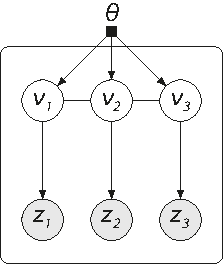
\includegraphics[width=\mywidtht]{ch-hvm/fig/hierarchical-variational-model.pdf}
    % \caption{\Acrlong{hvm}}%
    \label{fig:hvm-graphical-model}%
  \end{subfigure}
  \hspace*{\fill}%
  \begin{subfigure}[b]{\figwidtht}
    \centering
    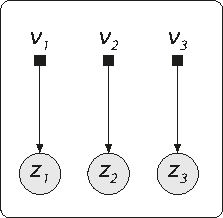
\includegraphics[width=\mywidtht]{ch-hvm/fig/mean-field-graphical-model.pdf}
    % \caption{Mean-field variational family}%
    \label{fig:mean field-graphical-model}%
  \end{subfigure}
  \hspace*{\fill}%
  % \vspace{-0.5cm}
  \caption[\textsc{hvm} and mean field approximation graphical models]{\textbf{\Acrlongpl{hvm} (\glspl{hvm}, left) capture dependencies between latent variables, compared to the mean field variational family with independent variables (right).}}
  \label{fig:graphical-model}
\end{figure}